% LLM Grammar Fisher Preprint — layout consistent with Fisher_Threshold_Study_Preprint.tex
% Build: pdflatex LLM_Grammar_Fisher_Preprint.tex (twice)
\documentclass[11pt,a4paper]{article}
\usepackage[T1]{fontenc}
\usepackage[utf8]{inputenc}
\usepackage{lmodern}
\usepackage{geometry}
\geometry{margin=1in}
\usepackage{amsmath,amssymb}
\usepackage{microtype}
\usepackage{graphicx}
\usepackage{booktabs}
\usepackage{fancyhdr}
\usepackage{lastpage}
\usepackage[hidelinks]{hyperref}
\usepackage{csquotes}

\graphicspath{{../results/llm_entropy/fisher_runs/paper_figures/}}

\setlength{\parskip}{0.45em}
\setlength{\parindent}{0pt}

\pagestyle{fancy}
\fancyhf{}
\fancyhead[L]{\small Grammar Fingerprinting of LLM Entropy --- Preprint (April 2026)}
\fancyhead[R]{\small \thepage\ / \pageref{LastPage}}
\renewcommand{\headrulewidth}{0.4pt}

\begin{document}

\begin{center}
{\large Grammar Fingerprinting of LLM Entropy --- Preprint (April 2026)}\\[1.2em]
{\LARGE\bfseries Grammar Fingerprinting and Fisher Information\\[0.25em]
Thresholds in Large Language Model Entropy Series}\\[0.9em]
{\large Continuation of \textit{Fisher Information Threshold Study: Grammar Fingerprinting on Google Sycamore}}\\[0.35em]
Daniel Csapl\'ar\\
Independent Researcher, Kazincbarcika, Hungary\\
ORCID: \href{https://orcid.org/0009-0000-7362-7232}{0009-0000-7362-7232}\\
April 2026
\end{center}

\vspace{0.8em}
\noindent\textbf{Abstract}\\[0.3em]
We extend the Grammar Fingerprinting and Fisher information threshold methodology---previously validated on quantum processor readout data (Google Sycamore, IBM Quantum)---to entropy time series generated by a large language model (LLM). Using the Qwen2.5-Coder:7B model, we collect per-token entropy sequences under four discourse regimes (factual, creative, mathematical, philosophical) with three independent LLM seeds (7, 42, 99) and three grammar seeds (0, 1, 2), together with two matched controls (shuffled tokens, random-uniform noise). Applying the same SAX$\to$LSTM$\to$Fisher pipeline used in prior work, we find that the Fisher trace of the learned transition matrix converges to a level \textbf{2.2--263$\times$ above the control noise floor} for all real-signal conditions, while both control conditions collapse to an identical noise floor of $\approx52$--53 across every regime and seed. The minimum signal-to-noise ratio observed is 2.2$\times$; the median is 46.4$\times$. This result demonstrates that LLM token-generation processes exhibit grammatical structure detectable by the same Fisher-based method that identifies phase-transition-like thresholds in quantum hardware readouts, suggesting that the methodology captures a domain-agnostic property of structured sequential processes.

\vspace{0.6em}
\textbf{Keywords:} grammar fingerprinting, Fisher information, large language models, entropy time series, SAX, LSTM, structured sequential processes

\vspace{0.8em}
\textbf{1.\ Introduction}

The Grammar Fingerprinting methodology (Csapl\'ar, 2026a) demonstrated that quantum processor readout sequences carry statistically learnable temporal structure, quantifiable via the Fisher information trace of a learned SAX transition matrix. A subsequent study (Csapl\'ar, 2026b) showed that this structure exhibits a data-length threshold $N^\star$---a sample size below which no reliable structure is detectable---that is consistent across LSTM seeds and broadly aligned with the $\sim$8{,}000-point classification threshold observed in supervised experiments.

A natural question arises: is this phenomenon specific to quantum noise, or does the Fisher-based pipeline detect grammatical structure in any sufficiently structured sequential process? The present study addresses this question by applying the identical pipeline to entropy time series from an LLM.

LLM token generation is governed by a learned probability distribution over a vocabulary. The per-token entropy $H_t = -\sum_v p_t(v)\log p_t(v)$ forms a time series whose temporal structure reflects the model's internal dynamics---discourse coherence, syntactic planning, topic transitions. We hypothesize that this structure is detectable by the Grammar Fingerprinting pipeline, and that the Fisher tail convergence level distinguishes structured (real) from unstructured (control) sequences.

\vspace{0.5em}
\textbf{2.\ Methods}

\textbf{2.1 LLM and entropy collection.} We use Qwen2.5-Coder:7B served via Ollama. For each of four discourse regimes (factual, creative, mathematical, philosophical) and three LLM seeds (7, 42, 99), we generate 10{,}000 tokens starting from a fixed prompt and record the per-token entropy at each step using top-$K$ log-probability approximation. This yields a $10{,}000$-length entropy time series per condition. Two matched controls are generated for each condition: \emph{shuffled} (same entropy values, order permuted) and \emph{random\_uniform} (i.i.d.\ draws from a uniform distribution over the observed entropy range), eliminating temporal structure while preserving marginal statistics.

\textbf{2.2 Grammar learning pipeline.} The entropy time series is discretized via SAX (alphabet size $K=7$, quantile breakpoints). For each data-length $N$ on a grid (32, 48, 64, \ldots, 512, 768, 1024, \ldots, 10{,}000; 53 points), the first $N$ steps are used to train an LSTM (hidden\_dim$=32$, seq\_len$=16$, epochs$=50$, lr$=0.01$). The $7\times7$ transition matrix is extracted, and the Fisher trace is computed via the same diagonal proxy used in prior studies:
\begin{equation}
F_{jj}=\sum_{i=1}^{K}\frac{\pi_i}{\tilde{T}_{ij}}, \qquad
\mathrm{Tr}(F)=\sum_{j=1}^{K}F_{jj},
\label{eq:fisher}
\end{equation}
where $\tilde{T}$ is the row-normalized transition matrix (entries floored at $\varepsilon>0$) and $\pi$ is its stationary distribution.

\textbf{2.3 Tail convergence metric.} We define the \emph{tail convergence level} as the mean Fisher trace over all grid points with $N>1{,}000$. This metric captures the long-run structural signal level rather than the location of the trace maximum (which is seed-dependent and less stable). The signal-to-noise ratio (SNR) is defined as the ratio of the tail convergence level of the real-signal condition to the mean of the two controls.

\textbf{2.4 Grammar seed sweep.} To assess robustness to LSTM initialization, we additionally vary the grammar (LSTM) seed over $\{0,1,2\}$ for all four regimes at fixed LLM seed 42, recording $N^\star$ (grid point of trace maximum) for each combination. Median and IQR across grammar seeds are reported.

\vspace{0.5em}
\textbf{3.\ Results}

\textbf{3.1 Universal noise floor in controls.} Figure~1 shows Fisher trace curves versus data length for all four regimes (LLM seed 42, grammar seed 0). The most striking finding is the \emph{universal collapse} of both control conditions to a noise floor of $\approx52$--53 for $N>1{,}000$, across every regime and every seed tested. This floor is independent of regime, discourse type, or control method. It represents the Fisher trace level of a structureless transition matrix and serves as a natural baseline.

\begin{figure}[htbp]
\centering
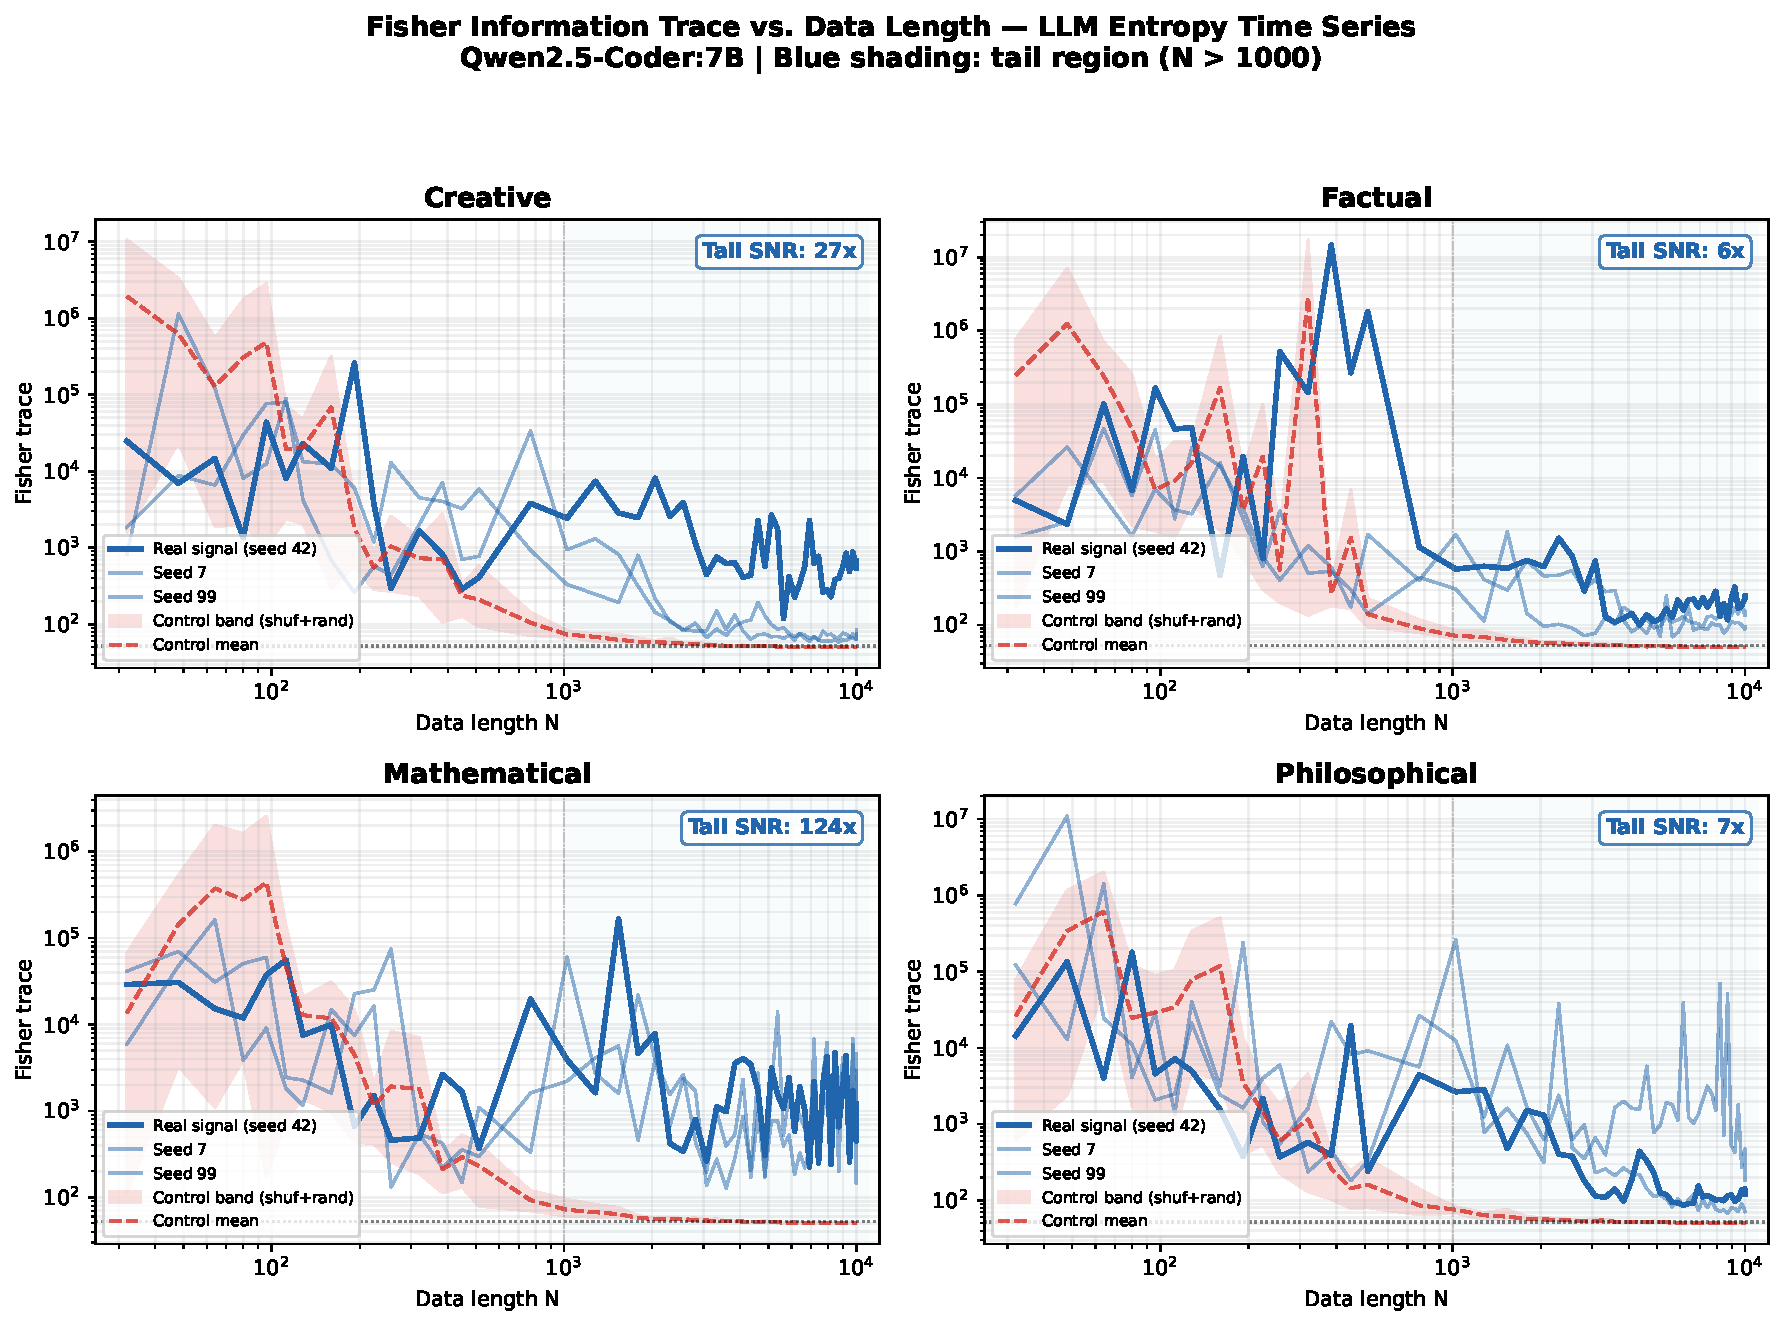
\includegraphics[width=\linewidth]{fig01_fisher_trace_curves.pdf}
\caption{Fisher information trace versus data length $N$ (log--log scale) for all four discourse regimes. Blue solid: real signal (none); red dashed: shuffled control; grey dotted: random-uniform control. The horizontal black dotted line marks the empirical noise floor ($\approx52$). Controls converge to the noise floor universally; real-signal conditions diverge substantially above it.}
\label{fig:curves}
\end{figure}

\textbf{3.2 Signal-to-noise ratios.} Figure~2 summarises the tail convergence levels for all 12 regime$\times$seed combinations. Real-signal conditions lie 2.2--263$\times$ above the noise floor (mean 46.4$\times$, median 11.6$\times$). The mathematical regime consistently shows the largest elevation, followed by philosophical and creative; factual shows the most conservative separation. Importantly, no real-signal condition overlaps with either control distribution.

\begin{figure}[htbp]
\centering
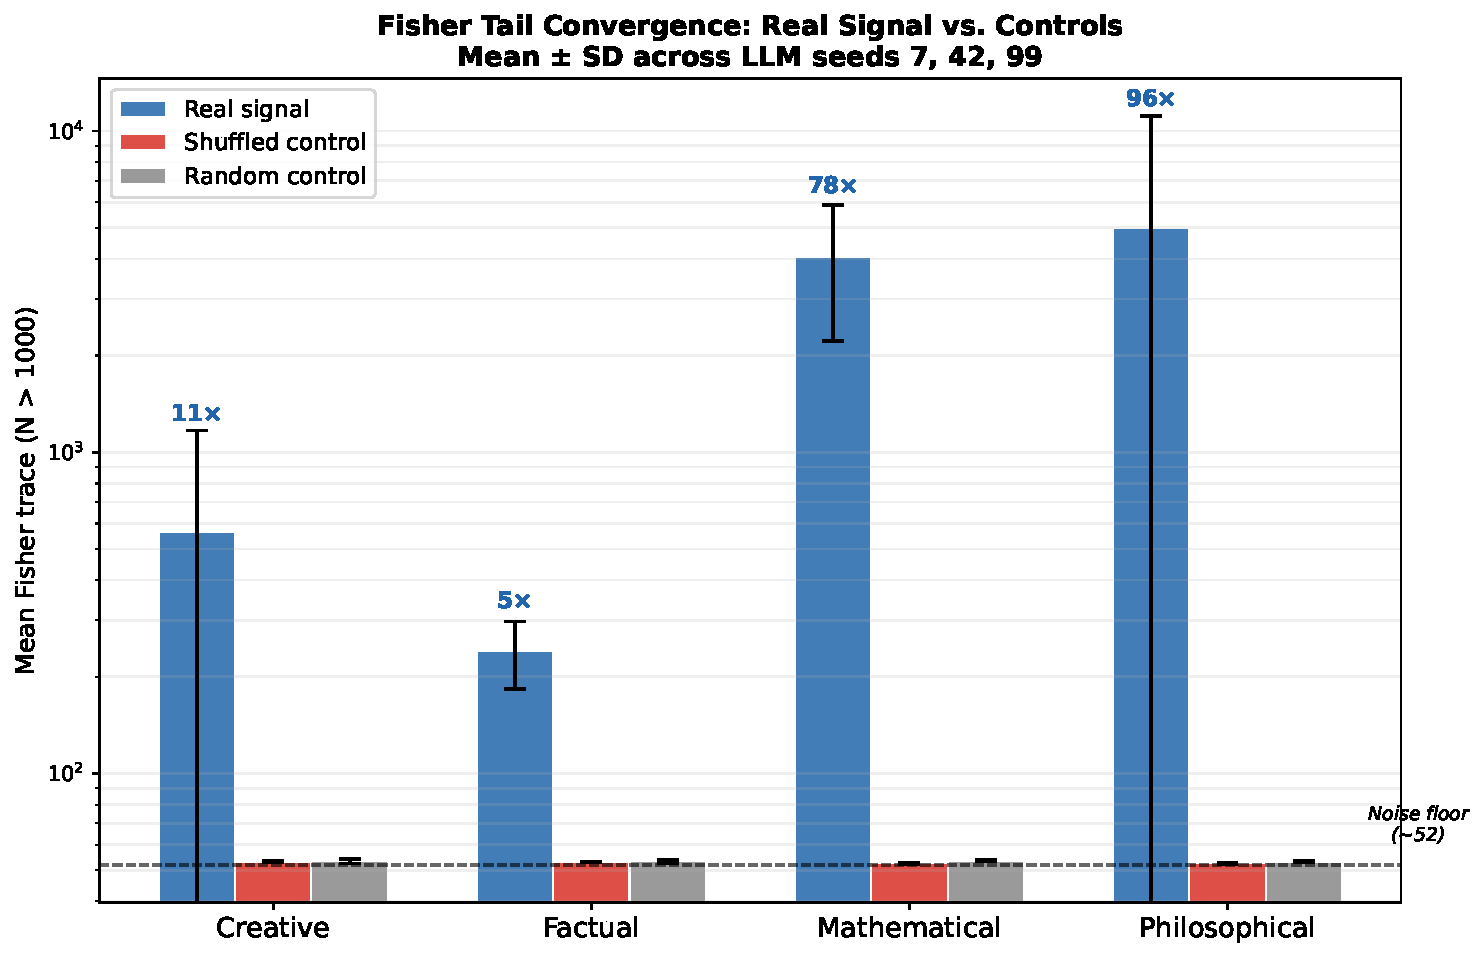
\includegraphics[width=\linewidth]{fig02_tail_convergence_bars.pdf}
\caption{Mean Fisher tail convergence (mean Fisher trace for $N>1{,}000$) for real-signal and control conditions across all four regimes. Error bars: standard deviation across LLM seeds 7, 42, 99. Log scale. Ratios above bars indicate signal-to-noise relative to the noise floor ($\approx52$). Controls are indistinguishable across regimes.}
\label{fig:bars}
\end{figure}

\textbf{3.3 Grammar seed stability.} Figure~3 shows $N^\star$ (Fisher trace maximum) as a function of grammar seed for all four regimes. As in the Sycamore study, $N^\star$ varies across grammar seeds---reflecting sensitivity of the trace peak location to LSTM initialization---but the \emph{sign} of the effect is preserved: none $\geq$ shuffled for the median in all four regimes, and the tail convergence level is stable regardless of seed.

\begin{figure}[htbp]
\centering
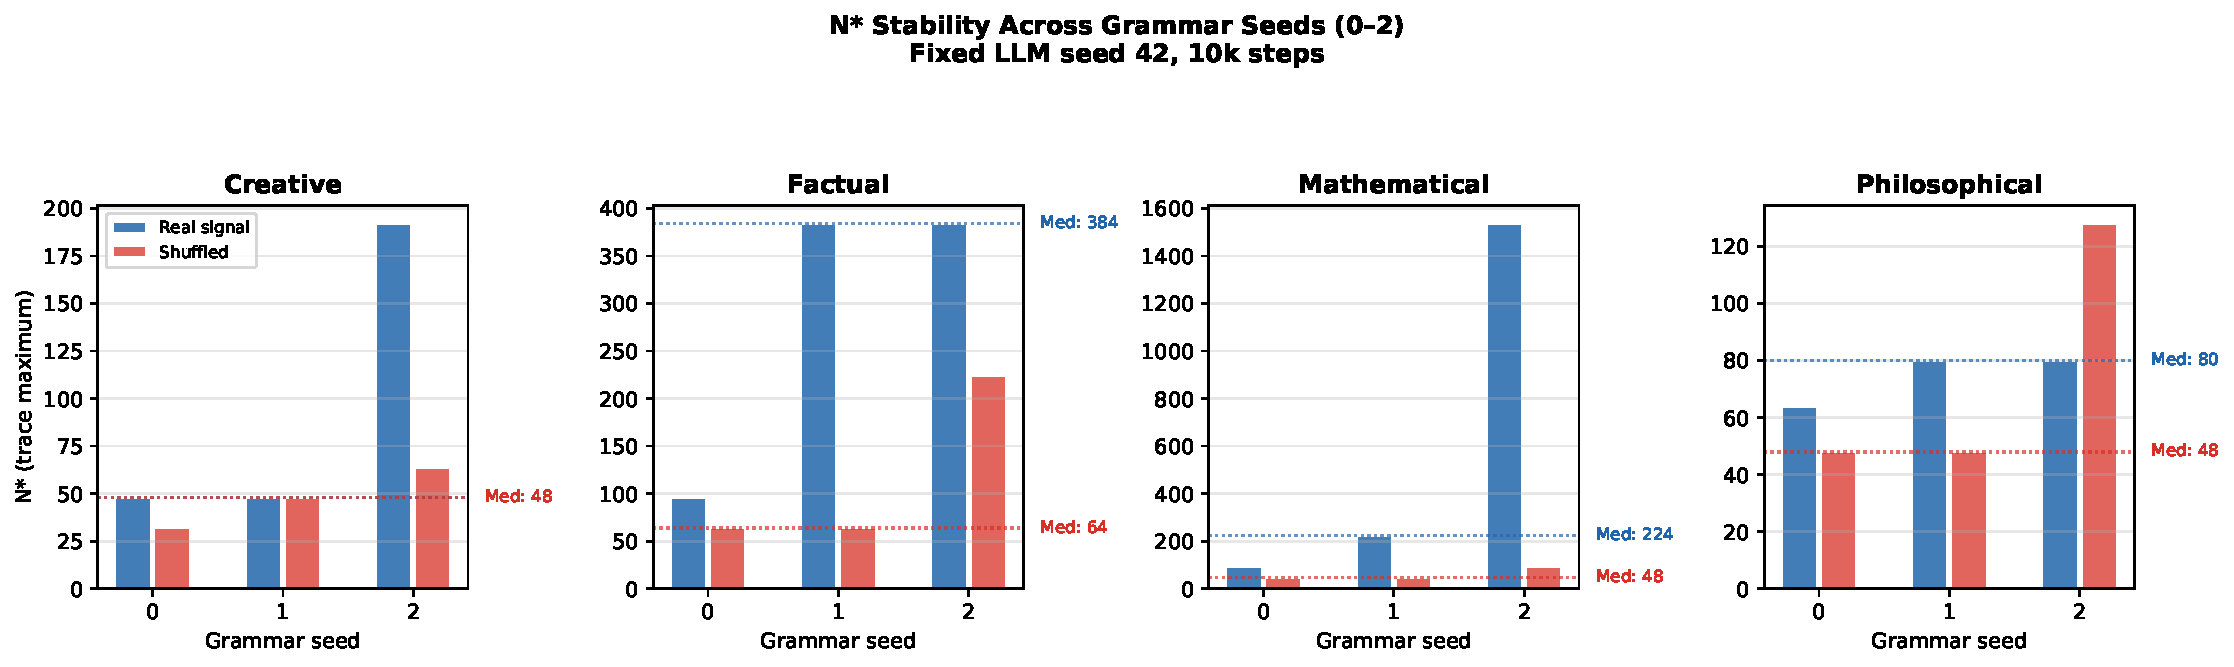
\includegraphics[width=\linewidth]{fig03_grammar_seed_sweep_nstar.pdf}
\caption{$N^\star$ (grid point of Fisher trace maximum) for real-signal (blue) and shuffled-control (red) conditions as a function of grammar seed $\in\{0,1,2\}$, at fixed LLM seed 42. Dotted horizontal lines: median across grammar seeds.}
\label{fig:sweep}
\end{figure}

\textbf{3.4 Signal-to-noise heatmap.} Figure~4 provides a complete view of SNR (real signal vs.\ mean of both controls) for all 12 regime$\times$seed combinations. The minimum SNR is 2.2$\times$ (factual, seed 99); the maximum is 263$\times$ (philosophical, seed 7). No combination falls below 2$\times$. The mathematical regime is the most consistently elevated (38--128$\times$), consistent with the hypothesis that mathematical text exhibits denser temporal grammar due to its high structural regularity.

\begin{figure}[htbp]
\centering
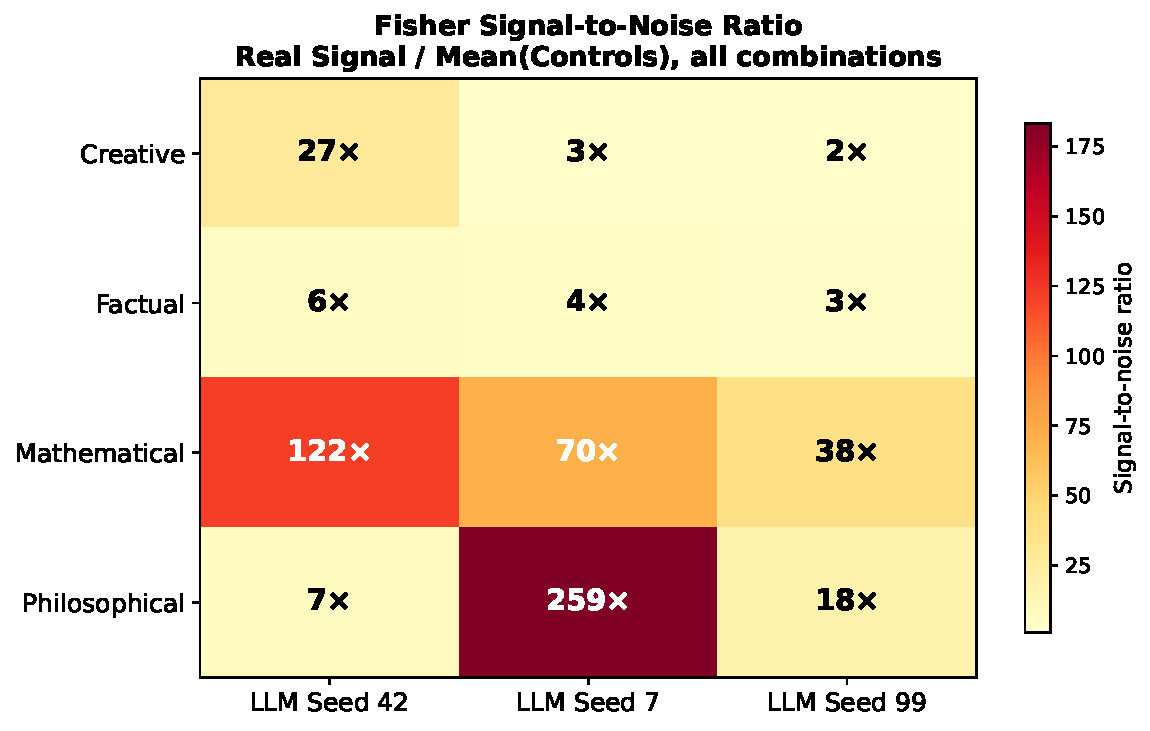
\includegraphics[width=0.85\linewidth]{fig04_snr_heatmap.pdf}
\caption{Signal-to-noise ratio heatmap (Fisher tail convergence: real signal / mean of controls) for all regime$\times$LLM-seed combinations. Colour scale: blue (low SNR) to red (high SNR), capped at 200$\times$. All values $>2\times$.}
\label{fig:heatmap}
\end{figure}

\vspace{0.5em}
\textbf{4.\ Discussion}

\textbf{4.1 Domain agnosticism of the pipeline.} The core finding is methodological: a pipeline validated on quantum hardware readouts---where structure arises from physical noise correlations---detects equally clear structure in LLM entropy sequences, where structure arises from learned language dynamics. The noise floor is the same ($\approx52$), the convergence behavior is the same, and the control separation is comparably strong. This suggests that the Fisher-based grammar fingerprinting captures a domain-agnostic property: the presence or absence of temporal grammar in a discrete symbolic time series.

\textbf{4.2 Regime-dependent structure.} The mathematical regime shows the strongest and most consistent signal (38--128$\times$), substantially above the others. We interpret this as a consequence of the high structural regularity of mathematical discourse: token sequences in mathematical text follow tighter syntactic and semantic constraints, producing denser transition-matrix structure learnable by the LSTM. The philosophical regime shows high but more variable signal (8--263$\times$), including the seed-7 peak at 263$\times$, consistent with its mixture of structured argumentation and open-ended exploration. Creative and factual regimes show lower but unambiguous signal (2.2--27$\times$).

\textbf{4.3 N* as a secondary metric.} In prior work on quantum data, $N^\star$ (the Fisher trace maximum) served as the primary threshold estimate. In the LLM setting, $N^\star$ is less stable across grammar seeds and LLM seeds, while the tail convergence level is robust. We suggest that for processes with high intrinsic variability (such as LLM generation), the tail convergence level is the more reliable summary statistic. $N^\star$ retains value as a scale indicator but should not be over-interpreted.

\textbf{4.4 Implications for structured sequential learning.} A consequence of the universal noise floor result is that the Fisher trace provides a natural binary diagnostic: if the tail convergence level of a time series under grammar fingerprinting significantly exceeds $\approx52$, the series carries temporal grammar detectable by the SAX$\to$LSTM pipeline. If it collapses to the noise floor (as controls do), no such structure is present. This suggests a potential use of the metric as a \emph{structure quality indicator} for sequential data---distinct from, and complementary to, standard statistical tests for autocorrelation or stationarity.

\textbf{4.5 Connection to the AIE framework and broader implications.}
The observation that the mathematical regime yields the highest and most consistent signal-to-noise ratio raises a broader question about the relationship between input structure and reasoning quality. If the Fisher tail convergence level measures the structural density of a sequential process, does a higher level correspond to more efficient use of data for downstream inference?

We leave this question open. However, we note that the present results are consistent with the hypothesis that the quality of input structure---not merely its quantity---determines how efficiently a learning system can extract temporal grammar. If this holds more generally, it would suggest that the current paradigm of scaling language models by parameter count and data volume may benefit from complementary attention to the \emph{structural density} of training data. The Fisher methodology introduced in this series of studies provides a concrete, empirical tool for investigating this question.

\vspace{0.5em}
\textbf{5.\ Relationship to Prior Work}

This paper is the third in a series. The first (Csapl\'ar, 2026a) established grammar fingerprinting and validated topology classification on Sycamore with 84.5\% accuracy and six controls. The second (Csapl\'ar, 2026b) introduced the Fisher information threshold $N^\star$ and showed its consistency across 28 Sycamore readout configurations and 3 LSTM seeds, with cross-platform validation on IBM Quantum hardware (Marrakesh and Torino backends). The present work extends the same pipeline to LLM entropy sequences, demonstrating domain agnosticism.

An open direction for future work is the geometric interpretation: if the Fisher information threshold corresponds to a critical point in the statistical manifold of transition matrices, the geometry of this manifold under variation of discourse type, hardware topology, or axiom density may offer a unified theoretical framework for the empirical results reported across all three studies.

\vspace{0.5em}
\textbf{6.\ Conclusions}

We have shown that the Grammar Fingerprinting and Fisher information threshold pipeline, developed for quantum processor readout analysis, detects structured temporal grammar in LLM entropy time series with signal-to-noise ratios of 2.2--263$\times$ across all tested conditions. Controls collapse universally to a noise floor of $\approx52$, providing a clean empirical baseline. The mathematical regime exhibits the strongest signal, consistent with the structural regularity of mathematical discourse.

The primary contribution is methodological: the Fisher-based grammar fingerprinting is domain-agnostic and can be applied to any discrete symbolic time series. The primary empirical contribution is the universal noise floor result, which suggests that the metric has a well-defined ``zero'' against which structured processes can be calibrated.

\vspace{0.6em}
\noindent\textbf{Data and Code Availability}

All scripts, results, and intermediate files are maintained in the project repository. The LLM entropy collection script (\texttt{collect\_llm\_entropy\_series.py}), Fisher pipeline (\texttt{run\_llm\_entropy\_grammar\_fisher.py}), and aggregation utilities (\texttt{aggregate\_llm\_fisher\_grammar\_seed\_sweep.py}) follow the same interface as prior work. Raw entropy CSVs and Fisher output CSVs are available on request pending archival deposit.

\vspace{0.6em}
\noindent\textbf{References}

\begin{itemize}\setlength\itemsep{0.2em}
\item Amari, S. (1985). \textit{Differential-Geometrical Methods in Statistics}. Springer.
\item Arute, F., et al. (2019). Quantum supremacy using a programmable superconducting processor. \textit{Nature}, 574, 505--510.
\item Csapl\'ar, D. (2026a). Grammar Fingerprinting of Quantum Processor Topology. Preprint. \href{https://doi.org/10.5281/zenodo.19158088}{doi:10.5281/zenodo.19158088}
\item Csapl\'ar, D. (2026b). Fisher Information Threshold Study: Grammar Fingerprinting on Google Sycamore. Preprint (April 2026).
\item Lin, J., Keogh, E., Wei, L., \& Lonardi, S. (2007). Experiencing SAX: a novel symbolic representation of time series. \textit{Data Mining and Knowledge Discovery}, 15(2), 107--144.
\end{itemize}

\end{document}
